%!TEX program = xelatex
%!TEX root = ./thesis.tex
\chapter{Methodology}
%!TEX program = xelatex
%!TEX root = ./thesis.tex
\section{Target Environments}\label{sec_env}
\subsection{Summary of Environment Design}
We propose and develop a set of tasks that are representatives of deep reinforcement learning environments with continuous action space, multi-modal state space and sparse reward functions. The design of the robots' physical systems is based on the 3D robot environments~\cite{roboschool_2018} in OpenAI Gym~\cite{openaigym}. The external environments and reward functions of the target tasks are different from the original environments in OpenAI Gym. There are three classes of 3D robot agents in the environments OpenAI Gym: Ant, Humanoid and Swimmer. The Ant agent is a quadruped robot with 8-dimensional action space, the Humanoid agent is a humanoid robot with 16-dimensional action space, and the Swimmer agent is a worm-like robot with 2-dimensional action space.  The three agents are shown in Figure~\ref{fig_agent_ant}, Figure~\ref{fig_agent_humanoid} and Figure~\ref{fig_agent_swimmer}.

We mainly focus on a set of different problems based on the Ant agent, because the agent has the capability of solving a rich variety of high-level tasks, while the learning of the agent's basic control skills is not too challenging. 
Compared to the Ant agent, the Swimmer agent is too simple and its capability of solving hierarchical tasks is limited. The Humanoid agent, on the other hand, has a much more unstable physical system compared to Ant, and poses too much difficulty in the learning basic locomotion skills.
\begin{figure}[H]
	
\includegraphics[width=0.5\textwidth]{images/agent_ant.png}
	\centering
	\caption{The Ant agent}\label{fig_agent_ant}
\end{figure}

\begin{figure}[H]
	
\includegraphics[width=0.5\textwidth]{images/agent_humanoid.png}
	\centering
	\caption{The Humanoid agent}\label{fig_agent_humanoid}
\end{figure}
\begin{figure}[H]
	
\includegraphics[width=0.5\textwidth]{images/agent_swimmer.png}
	\centering
	\caption{The Swimmer agent}\label{fig_agent_swimmer}
\end{figure}
%To provide a consistent comparison with other studies, the development of 
%!TEX program = xelatex
%!TEX root = ./thesis.tex

\subsection{Detailed Environment Specifications}
We provide a detailed description of the experiment environments in this section. All of the environments are based on the Ant task~\cite{openaigym}. 

In the original Ant task, the agent receives a 111-dimensional motion sensor input and produces an 8-dimensional action output. The input consists of a 13-dimensional vector that contains the robot's pose information, a 14-dimensional vector that represents its velocity information, and an 84-dimensional vector that contains contact force information. However, information about the agent's absolute position in the world map is not available.

For the proposed environments, the agent receives not only the 111-dimensional motion sensor input, but also a $64\times 64\times 1$ dimensional grayscale image observation. A sample image observation is shown in Figure~\ref{fig_ant_imgobs}. The image is not in a high resolution but is sufficient for the agent to observe the necessary information for the proposed tasks.

\begin{figure}[H]
	
\includegraphics{images/ant_imgobs.png}
	\centering
	\caption{A sample image observation of the target environments}
\end{figure}\label{fig_ant_imgobs}

A basic task, namely move0, is similar to the Ant environment in OpenAI Gym~\cite{openaigym}. The difference is that the state space has an extra image input. The agent is required to move in a specific direction $g_0=(1,0)$, and the reward at each time-step is given by:
\begin{align}
r = v_g + 1-c_p-c_c
\end{align}
where $v_g=v \cdot g_0$ is the forward reward, which rewards the agent for moving in the target direction. A spherical object presents in the environments at a constant distance from the robot agent to represent the target direction.  $c_p$ is the control cost, which is the power that the agent is consuming, and $c_c$ is the contact cost, which penalizes the agent for collisions. The episode terminates when the agent enters the unrecoverable state of being upside-down, or if the episode length reaches 1000 time-steps.

Apart from move0, a set of similar tasks with different target directions are denoted as move1, move2, move3, ..., move7. These tasks are similar to move0 because the goal direction is different. The image observation is actually redundant for all these low-level tasks, because the agent only needs to move in one specific direction in their corresponding environments. Snapshots of these source tasks are shown in Figure~\ref{fig:task8}.
\begin{figure}[!htbp]
	\centering
	\begin{subfigure}[t]{0.3\textwidth}
		\centering
		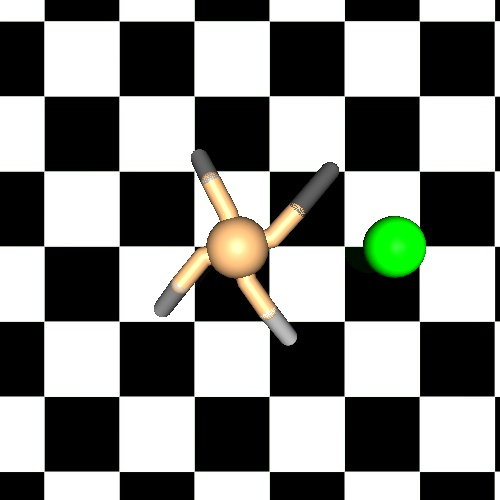
\includegraphics[width=\textwidth]{move0}
		\caption{move0}
	\end{subfigure}%
	~ 
	\begin{subfigure}[t]{0.3\textwidth}
		\centering
		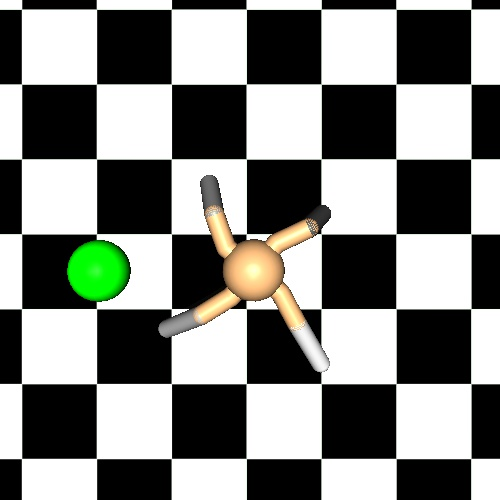
\includegraphics[width=\textwidth]{move1}
		\caption{move1}
	\end{subfigure}
	~ 
	\begin{subfigure}[t]{0.3\textwidth}
		\centering
		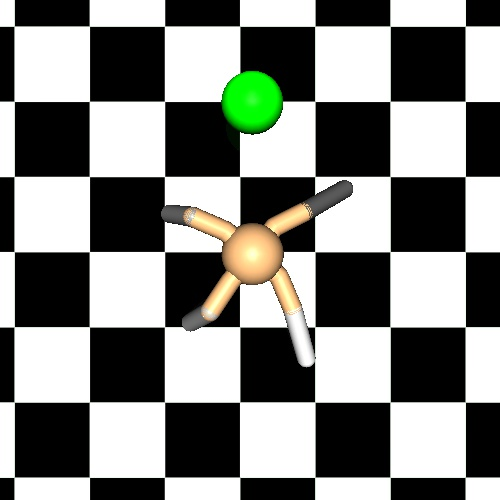
\includegraphics[width=\textwidth]{move2}
		\caption{move2}
	\end{subfigure}
	~ 
	\begin{subfigure}[t]{0.3\textwidth}
		\centering
		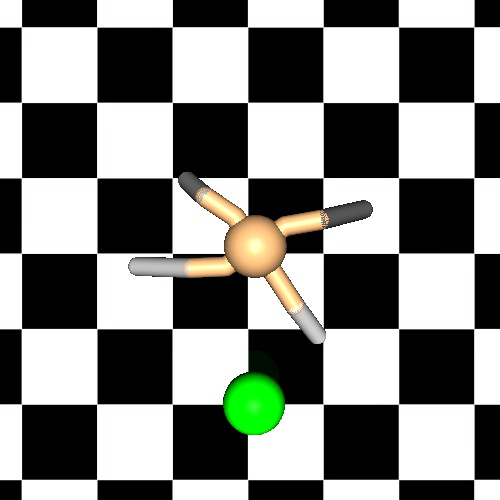
\includegraphics[width=\textwidth]{move3}
		\caption{move3}
	\end{subfigure}
	~ 
	\begin{subfigure}[t]{0.3\textwidth}
		\centering
		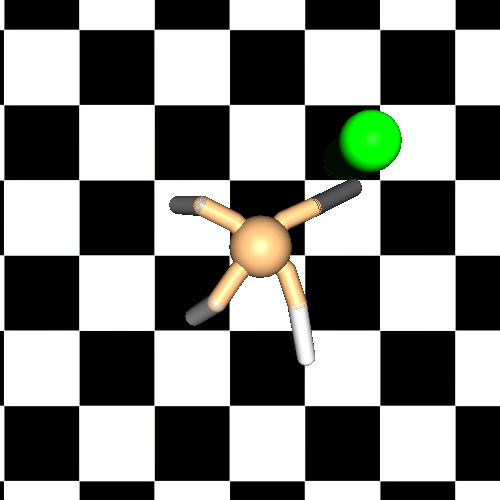
\includegraphics[width=\textwidth]{move4}
		\caption{move4}
	\end{subfigure}
	~ 
	\begin{subfigure}[t]{0.3\textwidth}
		\centering
		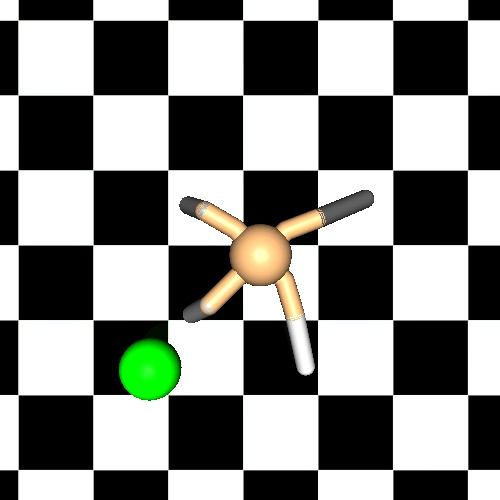
\includegraphics[width=\textwidth]{move5}
		\caption{move5}
	\end{subfigure}
	~ 
	\begin{subfigure}[t]{0.3\textwidth}
		\centering
		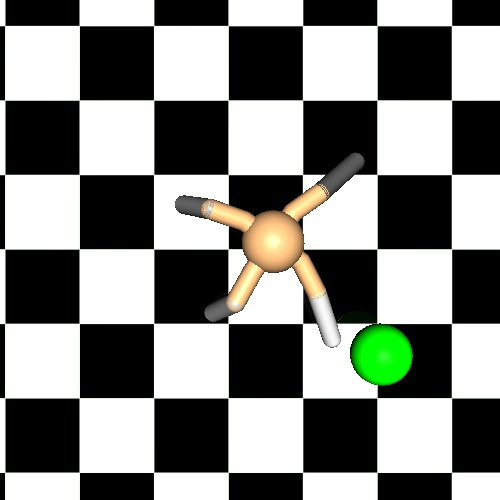
\includegraphics[width=\textwidth]{move6}
		\caption{move6}
	\end{subfigure}
	~ 
	\begin{subfigure}[t]{0.3\textwidth}
		\centering
		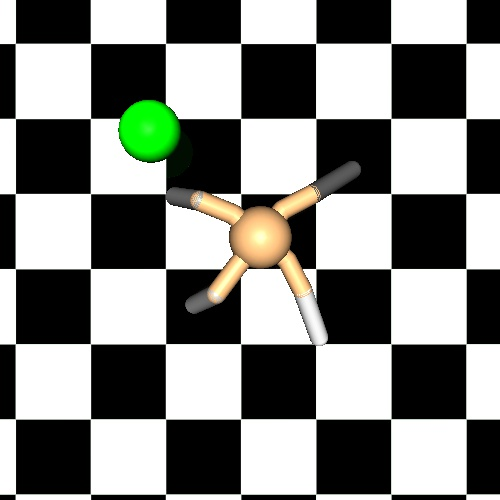
\includegraphics[width=\textwidth]{move7}
		\caption{move7}
	\end{subfigure}

	\caption{The source tasks}
	\label{fig:task8}
\end{figure}

Apart from these simple task, we also propose a set of tasks with more complexity. We propose several tasks with multi-modal state spaces such as moveg2, movecont, dynamicg8. These tasks require the agent to learn not only from the state representation but also the image representation. We also propose several more challenging tasks which has sparse reward fucntions, such as reachcont. The agent receives sparse reward signals in these environments. The target direction or location is represented by a spherical object and can be seen in the image observation.
The set of all the proposed environments are described in details in table \ref{table_ant_envs}.


\begin{table}[!htbp]

\begin{center}
\begin{tabular}{|c|p{3cm}|p{4cm}|p{4cm}|}
\hline
Task name & Goal & Reward  &  Description \\
\hline\hline
move0 & velocity: $g_0=(1,0)$ &$ v_g+1-c_p-c_c$  & move in a target direction \\
\hline
move1 & velocity: $g_1=(-1,0)$ &$ v_g+1-c_p-c_c$  & move in a target direction\\
\hline
move2 & velocity: $g_2=(0,1)$ &$ v_g+1-c_p-c_c$  & move in a target direction \\
\hline
move3 & velocity: $g_3=(0,-1)$ &$ v_g+1-c_p-c_c$  & move in a target direction \\ 
\hline 
move4 & velocity: $g_4=(\sqrt{2}/2,\sqrt{2}/2)$ &$ v_g+1-c_p-c_c$  & move in a target direction \\ 
\hline 
move5 & velocity: $g_5=(-\sqrt{2}/2,-\sqrt{2}/2)$ &$ v_g+1-c_p-c_c$  & move in a target direction \\ 
\hline 
move6 & velocity: $g_6=(\sqrt{2}/2,-\sqrt{2}/2)$ &$ v_g+1-c_p-c_c$  & move in a target direction \\ 
\hline 
move7 & velocity: $g_7=(-\sqrt{2}/2,\sqrt{2}/2)$ &$ v_g+1-c_p-c_c$  & move in a target direction \\ 
\hline 
moveg2 & velocity samples from: $\{g_0,g_1\}$ &$ v_g+1-c_p-c_c$  & each episode has a random sampled target direction \\ \hline
%moveg4 & velocity samples from: $\{g_0,g_1,g_2,g_3\}$ &$ v_g+1-c_p-c_c$  & each episode has a random sampled target direction \\ \hline
%moveg8 & velocity samples from: $\{g_0,g_1, \dots,g_7\}$ &$ v_g+1-c_p-c_c$  & each episode has a random sampled target direction \\ \hline
movecont & velocity samples from the unit circle&$ v_g+1-c_p-c_c$  & each episode has a random sampled target direction \\ \hline
dynamicg8 &  velocity samples from: $\{g_0,g_1, \dots,g_7\}$ &$ v_g$  & the target direction is re-sampled with probability 0.005 at each time-step  \\ \hline
%dynamiccont & velocity samples from a continuous range of all unit directions &$ v_g$  & the target direction is re-sampled with probability 0.005 at each time-step  \\ \hline
%reachg4 & position samples from $\{g_0,g_1,g_2,g_3\}$ & $I(\lVert x-g\rVert_2^2<0.5) - 0.01$  & The agent is terminated when reaching a target position\\ \hline
reachcont & position samples from the unit circle & $I(\lVert x-g\rVert_2^2<0.5) - 0.01$  & the episode is terminated when reaching a target position\\ \hline
reachcontreg & position samples from the unit circle & $5I(\lVert x-g\rVert_2^2<0.5) - 0.01$  & a new target is sampled and the episode continuous once the target position is reached\\ \hline
constdirreachreg & target direction samples from: $\{g_0,g_1, \dots,g_7\}$ & $5I(x_g > 1) - 0.01$  & a reward is given once the agent has moved in the target direction for a constant distance, then a new target is sampled\\ \hline
\end{tabular}
\end{center}
 \caption{Specification of the tasks}
\end{table}\label{table_ant_envs}




%!TEX program = xelatex
%!TEX root = ./thesis.tex
\section{Wasserstein Actor Critic Kronecker-factored Trust Region Policy Optimization Method }
As is reported in \cite{henderson2017matters}, the result of the current state-of-art deep reinforcement learning methods for continuous control, including TRPO, ACKTR, PPO and DDPG are difficult to be reproduced, due to they're heavily influenced by a variety of factors including random seed, neural network architecture, activation functions of neural network layers and even software implementation. This fact has reduced the reliability of these methods, and introduces difficulty in comparing their performance.

Particularly, the reproducibility problem with trust region methods including TRPO and ACKTR could be due to the training gets stuck in local minimum states. These trust region method has a naturally decreasing learning rate due to the KL-divergence measure. 

We propose a new policy optimization method, namely Wasserstein Actor Critic Kronecker-factored Trust Region Policy Optimization (W-KTR), in order to achieve a better performance on the proposed tasks, in terms of the agent's final performance, total training time and reproducibility.

The proposed W-KTR method focus on the problem scope of deep reinforcement learning for continuous control, specifically robot control problems. The physical meaning of action of these environments usually stands for mechanics-related physical quantity, such as motor torque and target motor phase. However, the traditional KL-divergence based trust region algorithms may not be suitable for these problems. Because the KL-divergence only focus on the intersection of policy distributions and may not be a good measure of the deviation of policy. A small perturbation in the mean value of a policy with Gaussian distribution from 1.0 to 1.01 will lead to a large KL-divergence when the variance has a small value such as 0.003. However, the perturbation may not lead to a significant difference in reality.

Therefore, we propose to use the Wasserstein metric, to measure the deviation of the policy updates. The Wasserstein metric as a trust region criteria has also been studied in previous literature~\cite{tolstikhin2017wasserstein}. We reformulate the trust region policy optimization problem as follows:
\begin{equation}
    \begin{aligned}
&    \underset{\theta}{\text{maximize}} 
&& J(\theta) \\
& \text{subject to } 
&& \overline{W_2}(\pi_{\theta_{old}},\pi_\theta) \leq \delta_{W}\end{aligned}
\end{equation}
where $ \overline{W_2}(\pi_{\theta_{old}},\pi_\theta)$ is the average Wasserstein-2 metric between the old policy and the current policy.

The Wasserstein-2 metric is defined by the following equation \cite{villani2003topics}:
\begin{equation}
    W_2(P,Q) = 
    \inf_{\Gamma \in \mathbb{P}(X \sim P, Y \sim Q)}
    \mathbb{E}_{X,Y \sim \Gamma} \left[ \lVert X-Y \rVert_2^2 \right]^{1/2}
\end{equation}
where $\mathbb{P}(X \sim P, Y \sim Q)$ is the set of all joint distribution of $X,Y$ with marginals $P,Q$ respectively.

Specifically, when $P$ and $Q$ are Gaussian distributions with mean $m_1,m_2$ and covariance matrix $\Sigma_1$ and $\Sigma_2$, the squared value of Wasserstein-2 distance $W_2^2(.)$ is defined as the following equation~\cite{chafai} :
\begin{equation}
    W_2^2(P,Q) = \Vert m_1-m_2\Vert_2^2 +\mathrm{Tr}\left(\Sigma_1+\Sigma_2-2(\Sigma_1^{1/2}\Sigma_2\Sigma_1^{1/2})^{1/2}\right)
\end{equation}

The problem is solved by performing gradient updates iteratively following the natural gradient with the Rianmanian metric as $W_2$ metric:

\begin{equation}
    s=H_\theta\left( \overline{W_2^2}(\pi_{old},\pi) \right)^{-1}g := A^{-1}g
\end{equation}
%
%We use the approximation of the Rianmanian metric tensor A:
%
%\begin{equation}
%    A \approx \mathbb{E}_{s_t} \left[
%    \nabla_\theta W_2^2(\pi_{old},\pi) \left(\nabla_\theta W_2^2(\pi_{old},\pi) \right)^T
%    \right]
%\end{equation}
If the non-diagonal entries in covariance matrices are all zero, the metric $W_2^2(.)$ is simply a second order term over the means and the square root of the covariance matrices:
\begin{equation}
W_2^2(P,Q) = \Vert m_1-m_2\Vert_2^2 +\Vert \Sigma_1^{1/2}-\Sigma_2^{1/2}\Vert_2^2
\end{equation}
The metric can actually be represented as a squared error between two parameter vectors:
\begin{equation}
W_2^2(P,Q) = \Vert \text{vec}[m_1,diag(\Sigma_1^{1/2})]-\text{vec}[m_2,diag(\Sigma_2^{1/2})]\Vert_2^2 
\end{equation}
The solution of this kind of expressions can then be computed using the Kronecker-factor approximation technique~\cite{wu2017scalable}.

The policy is then updated following the gradient direction $s$ with ADAM stochastic optimization algorithm~\cite{kingma2014adam}. The step size is adjusted in an adaptive manner according to the resulting $W_2$ distance at each training step.
\section{Hierarchical reinforcement learning architecture}
We propose to solve the reinforcement learning problem by a two-level hierarchical model. 

The hierarchical model consists of a top-level decider agent and a set of bottom-level actuator agents. The actuator agents' policies are trained from the source task environments. 

The decider agent takes an action at every time-step. It may either decide which source-task sub-policy should be executed, or simply skip and continue current sub-policy. Therefore, assume there are $a$ sub-policies, the action space of the root agent is an $(a+1)$-discrete action space.

The observation space of the root agent consists of 2 parts, original observation (motion-sensor observation, image observation) and meta observation. The meta observation indicates the current sub-policy being executed.

The selected leaf agent executes the corresponding sub-policy and computes the primary actions the agent should take for the original environment.

 The overalll decision-making process of the decider agent is shown in Algorithm~\ref{hrl_decision_proc}.

\begin{algorithm}
\caption{The decider agent mechanism}\label{hrl_decision_proc}
\begin{algorithmic}%[1]
\Function{deciderAct}{self,$s_t$}
\State $a_{decider} \sim \pi_{decider}(s_t)$
 \If{$a_{decider} \neq 0$}
 \State $self.currentActuator \gets self.allA
ctuators[a_{decider}-1]$
 \EndIf
\State $a_{actuator} \gets self.currentActuator.act(s_t)$
\State \Return $a_{actuator}$
\EndFunction
\end{algorithmic}
\end{algorithm}

\section{Generalized advantage estimation for hierarchical reinforcement learning agents}


% \section{Ensuring robustness on the transferred source-task policy}
% It is likely that the state distribution of the target task could be different from the source task environments even if the state-transition dynamics are the same. As a result, the source-task sub-policy may have bad performance in the target environment if it is not robust enough.

% \subsection{Domain randomization~\cite{tobin2017domain}}
% The first solution to the problem is to introduce more variance in the initial-state distribution when training the sub-policy in the source environment. However, this method may not guarantee the robustness.
% \subsection{Train the subpolicies from scratch in the target environment with true source-task reward functions}
% Training the subpolicies from scratch in the target tasks can avoid the problem of transfer learning. However, the method is not efficient and not applicable to general target tasks.
% \subsection{Fine-tuning the trained subpolicies using the true source-task reward functions}
% Another method can be training the source-task policy in the target environment with a fixed uniform root agent. That will require the reward function of the source environments to be known when training in the target environment.

% \subsection{Fine-tuning the subpolicies using a trained Q-function}
% A proposal is to train a Q-function during the training of the source task, and then fine-tune the policy using the trained Q-function and V-function when learning the target task. This method would require the learned Q-function to be sufficiently robust.

% \subsection{Training extra subpolicies to handle subpolicy switching}
% One way to deal with the problem is to fix the subpolicies and train an extra subpolicy that is executed between the switch of the policies

% \section{Automatic Learning of the termination policy of source-task sub-policies}


% \subsection{Model architecture}
% The architecture of the full root policy is shown in the below equations:

% \begin{equation}
%     c = k_{c}\sigma(\pi_{c}(s)+w_i(b_i-t_{ex}))
% \end{equation}
% \begin{equation}
%     \pi_{final} = (1-c)(\pi(s))
% \end{equation}
     

% In the equations, $c$ denotes the probability to continue the currently executed sub-policy, which is a Sigmoid function. $\pi_{c}(s)$ is a neural network model that takes the observation as input. When $\pi_{c}(s)$ is small and $w_i$ is large, the termination policy will basically be a fixed length termination criteria with length $b_i$.


% The root agent terminates the current sub-policy with probability (1-c) and makes the decision according to $\pi(s)$.

% \subsection{Loss function}
% A penalty should be added to the original loss function in the policy gradient algorithm. The objective is to make the decision points of the root agent sparse.

% A proposal is to use the sum-of-likelihood value of the "continue" action. The problem of this loss is that it will be influenced largely by the values near 0.

% An alternative is to add penalty if the root agent doesn't change the sub-policy to be executed although it terminates the original sub-policy and makes the decision again. However, this makes the objective non-stationary.

% \subsection{Coordination between the termination policy training and decision policy training}

% It is obvious that a trainable termination policy introduces an extra source of complexity. Simultaneous training on the root decision policy and termination policy may not work.

% A proposed method is to initialize the fixed length termination policy initially, then train the two models in an alternating manner.